\documentclass[a4paper, 11pt]{article}
\usepackage{comment} % enables the use of multi-line comments (\ifx \fi) 
\usepackage{lipsum} %This package just generates Lorem Ipsum filler text. 
\usepackage{fullpage} % changes the margin
\usepackage{graphicx}

\begin{document}
%Header-Make sure you update this information!!!!
\noindent
\large\textbf{Lab Report 2} \hfill \textbf{Bryant Hayes} \\
\normalsize Applied Robotics \hfill Teammates: Bryan Bowman, Taylor Rawlings \\

\section*{Individual Progress}
I have made a lot of progress the last few weeks. A lot of time was initially put into getting the inverse kinematics working for the robotic arm with the goal of being able to move a palletizing style arm accurately in XYZ coordinates. This was a critical piece of our project because without it, all the other work would be for nothing. After getting that to work with our new I2C PWM board, I focused on working with our mechanical engineer to finish the hardware and structure design, so that I could start testing the camera and getting all the electronics mounted to the chassis. At this point we have gotten the entire robot built and now only code remains for the most part.\\

\begin{figure}[h]
	\caption{Camera algorithms find keypoint locations}
	\centering
	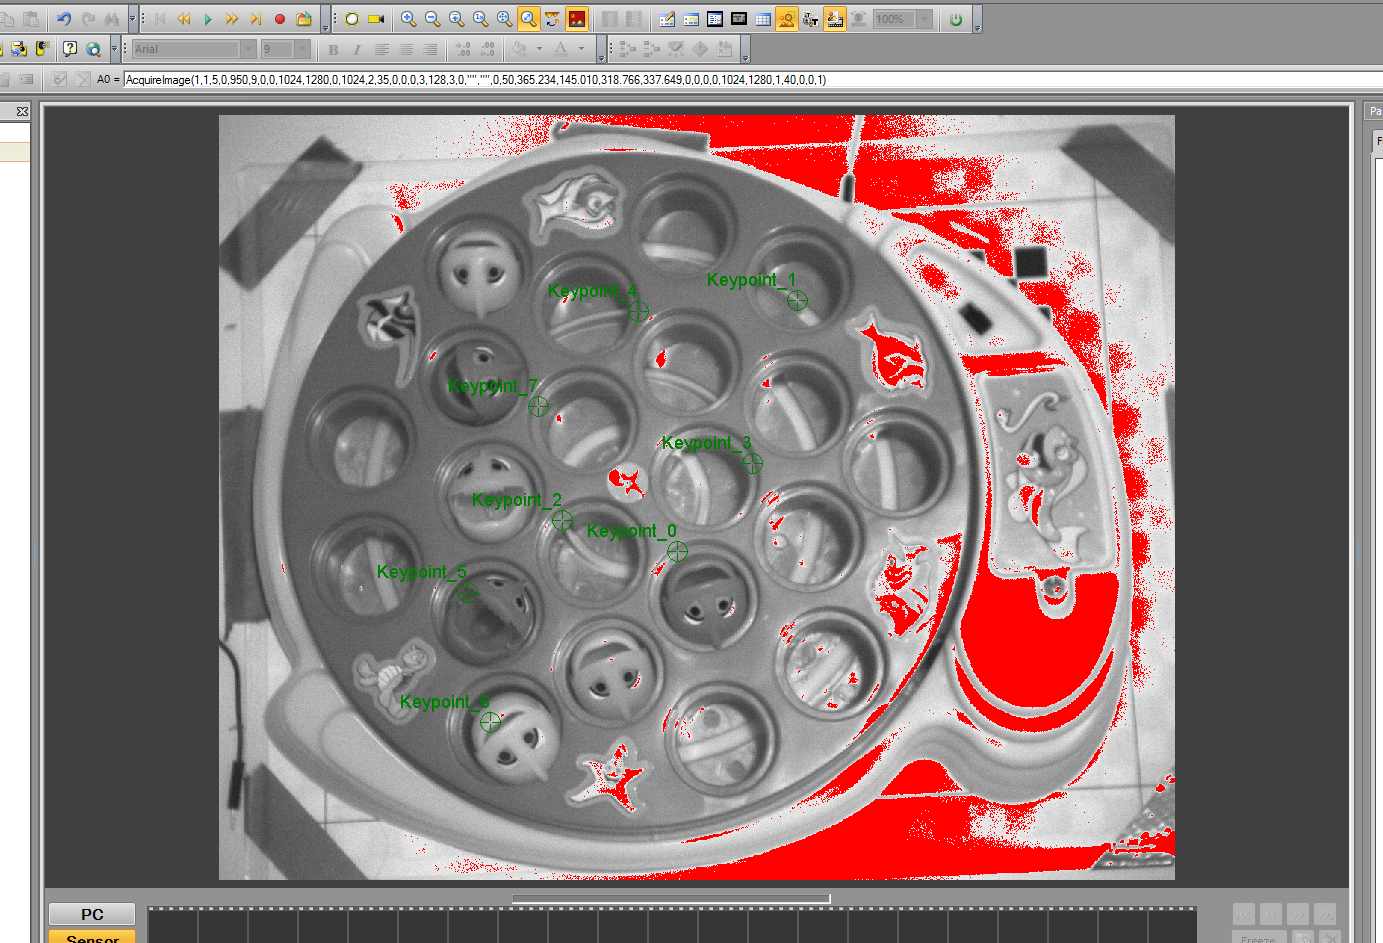
\includegraphics[width=0.75\textwidth]{Capture}
\end{figure}

\noindent On the camera side, I was able to get the current board orientation, board rotational speed and board XYZ coordinates in real time. Our Cognex In-Sight 7000 cameras are really quite amazing and easy to use. There was a bit of trig and math involved in getting the location of all the key-points based on the current board position and orientation, but I managed to get it working pretty accurately.

\section*{Challenges/Issues}
One major challenge was getting communication between the In-Sight 7000 camera system and our microprocessor. I spent probably 12 hours trying to get it to work without any progress. In the end, what we thought was a ground wire, wasn't. This was why all our data wasn't making sense, and once we got it wired up correctly it worked almost right away.\\

\noindent Another challenge we faced was when one of our original servos broke and cause a short, shutting down our microprocessor. This was handled by switching to better servos, which required a lot of extra work. In the long run however, I think the new servos are worth it.

\section*{Relate to Team Goals}
I have tried to make sure that my current task is always one that will advance our progress the most. I think I have done well in prioritizing my time so that we were able to keep our momentum and get a lot done each week. I have also made an effort to have weekly meetings to schedule everyones tasks and goals.

\section*{Goals for the week}
This week's goal is to finish the camera/Edison communication and hopefully get our first fish autonomously. We believe we have all the necessary components, I just need to write the code to control the state machine and logic our robot will follow.

% \begin{thebibliography}{9}
% \bibitem{Robotics} Fred G. Martin \emph{Robotics Explorations: A Hands-On Introduction to Engineering}. New Jersey: Prentice Hall.
% \bibitem{Flueck}  Flueck, Alexander J. 2005. \emph{ECE 100}[online]. Chicago: Illinois Institute of Technology, Electrical and Computer Engineering Department, 2005 [cited 30
% August 2005]. Available from World Wide Web: (http://www.ece.iit.edu/~flueck/ece100).
% \end{thebibliography}

\end{document}